\documentclass[12pt,notitlepage]{article}
\pagestyle{empty}
\usepackage[lmargin=1.5in,rmargin=1in,tmargin=1in,bmargin=1in]{geometry}                % See geometry.pdf to learn the layout options. There are lots.
\geometry{letterpaper}                   % ... or a4paper or a5paper or ... 
%\geometry{landscape}                % Activate for for rotated page geometry
%\usepackage[parfill]{parskip}    % Activate to begin paragraphs with an empty line rather than an indent
\usepackage{parskip}
\usepackage{graphicx}
%\usepackage{amssymb}
%\usepackage{epstopdf}
%%
%\usepackage{rotating}
%\usepackage{tikz}
%\usetikzlibrary{shapes,arrows}
%\usepackage{graphicx}
%\usepackage{tikz-dependency}
\usepackage{natbib}
\usepackage{url}
\usepackage{color,soul}
\usepackage{multirow}
\usepackage{fancyhdr}

%\DeclareGraphicsRule{.tif}{png}{.png}{`convert #1 `dirname #1`/`basename #1 .tif`.png}
\setlength{\parindent}{15pt} %Paragraphs will not be indented
%\parskip=10pt
\linespread{1.2}

%\title{PDT items}
%\author{Levi King \\ Last updated:}
\date{}

%%\pagestyle{fancy}
%%\fancyhf{}
%%\fancyhead[C]{\textbf{PDT Items}}
%%\renewcommand{\headrulewidth}{0pt}
%\fancyhead[RE,LO]{Guides and tutorials}
%\fancyfoot[CE,CO]{\leftmark}
%\fancyfoot[LE,RO]{\thepage}
\begin{document}
%\maketitle

\begin{center}

{\Large \textbf{PDT Items}}

\vspace{2em}

\begin{tabular}{|c|c|c|}
\hline
01 (In): What is the boy doing? && 02 (Tr): What is the boy doing? \\
\hline

\includegraphics[width=16em,trim=0 0 0 -3]{figures/I01.jpg} & & 
\includegraphics[width=16em,trim=0 0 0 -3]{figures/I02.jpg} \\
\hline
\end{tabular}
\vspace{1em} \\


\begin{tabular}{|c|c|c|}
\hline
03 (Di): What is the man doing? && 04 (In): What is the boy doing? \\
\hline
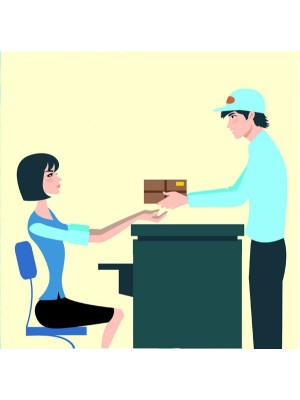
\includegraphics[width=16em,trim=0 0 0 -3]{figures/I03.jpg} & & 
\includegraphics[width=16em,trim=0 0 0 -3]{figures/I04.jpg} \\
\hline
\end{tabular}
\vspace{1em} \\

\clearpage

{\Large \textbf{PDT Items}}

\vspace{2em}

\begin{tabular}{|c|c|c|}
\hline
05 (Di): What is the teacher doing? && 06 (Tr): What is the boy doing? \\
\hline
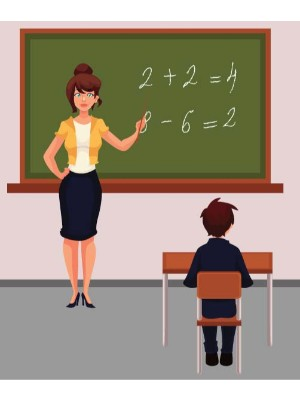
\includegraphics[width=16em,trim=0 0 0 -3]{figures/I05.jpg} & & 
\includegraphics[width=16em,trim=0 0 0 -3]{figures/I06.jpg} \\
\hline
\end{tabular}
\vspace{1em} \\


\begin{tabular}{|c|c|c|}
\hline
07 (In): What is the bird doing? && 08 (Di): What is the waiter doing? \\
\hline

\includegraphics[width=16em,trim=0 0 0 -3]{figures/I07.jpg} & & 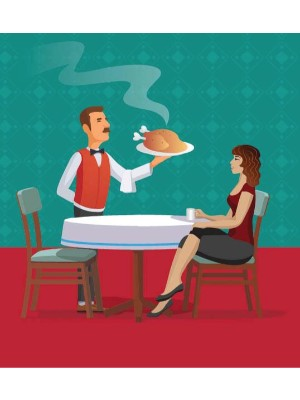
\includegraphics[width=16em,trim=0 0 0 -3]{figures/I08.jpg} \\
\hline
\end{tabular}
\vspace{1em} \\


\clearpage

{\Large \textbf{PDT Items}}

\vspace{2em}

\begin{tabular}{|c|c|c|}
\hline
09 (Tr): What is the girl doing? && 10 (In): What is the baby doing? \\
\hline
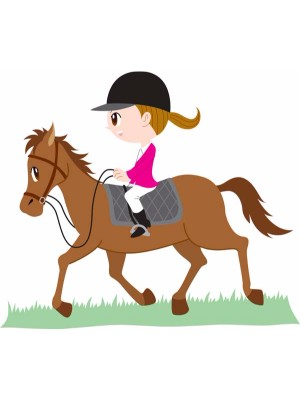
\includegraphics[width=16em,trim=0 0 0 -3]{figures/I09.jpg} & & 
\includegraphics[width=16em,trim=0 0 0 -3]{figures/I10.jpg} \\
\hline
\end{tabular}
\vspace{1em} \\


\begin{tabular}{|c|c|c|}
\hline
11 (Di): What is the boy doing? && 12 (Tr): What is the woman doing? \\
\hline
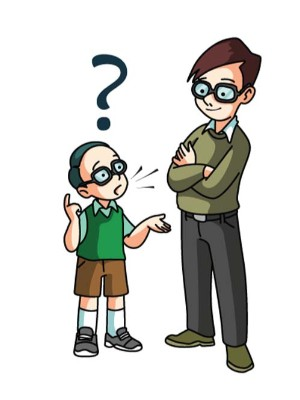
\includegraphics[width=16em,trim=0 0 0 -3]{figures/I11.jpg} & & 
\includegraphics[width=16em,trim=0 0 0 -3]{figures/I12.jpg} \\
\hline
\end{tabular}
\vspace{1em} \\


\clearpage

{\Large \textbf{PDT Items}}

\vspace{2em}

\begin{tabular}{|c|c|c|}
\hline
13 (In): What is the man doing? && 14 (Di): What is the man doing? \\
\hline

\includegraphics[width=16em,trim=0 0 0 -3]{figures/I13.jpg} & & 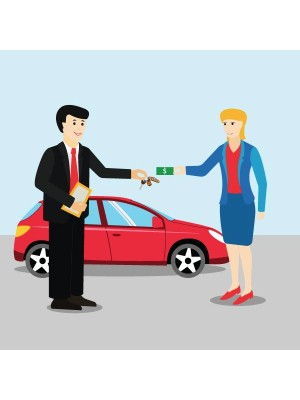
\includegraphics[width=16em,trim=0 0 0 -3]{figures/I14.jpg} \\
\hline
\end{tabular}
\vspace{1em} \\


\begin{tabular}{|c|c|c|}
\hline
15 (Tr): What is the man doing? && 16 (Tr): What is the frog doing? \\
\hline

\includegraphics[width=16em,trim=0 0 0 -3]{figures/I15.jpg} & & 
\includegraphics[width=16em,trim=0 0 0 -3]{figures/I16.jpg} \\
\hline
\end{tabular}
\vspace{1em} \\


\clearpage

{\Large \textbf{PDT Items}}

\vspace{2em}

\begin{tabular}{|c|c|c|}
\hline
17 (Di): What is the girl doing? && 18 (In): What is the man doing? \\
\hline
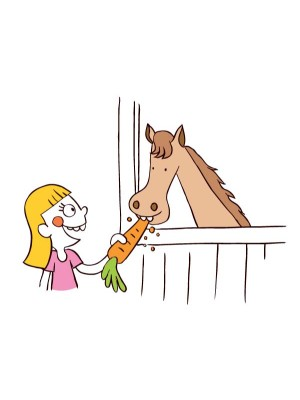
\includegraphics[width=16em,trim=0 0 0 -3]{figures/I17.jpg} & & 
\includegraphics[width=16em,trim=0 0 0 -3]{figures/I18.jpg} \\
\hline
\end{tabular}
\vspace{1em} \\


\begin{tabular}{|c|c|c|}
\hline
19 (Tr): What is the woman doing? && 20 (In): What is the girl doing? \\
\hline

\includegraphics[width=16em,trim=0 0 0 -3]{figures/I19.jpg} & & 
\includegraphics[width=16em,trim=0 0 0 -3]{figures/I20.jpg} \\
\hline
\end{tabular}
\vspace{1em} \\


\clearpage

{\Large \textbf{PDT Items}}

\vspace{2em}

\begin{tabular}{|c|c|c|}
\hline
21 (Di): What is the boy doing? && 22 (Tr): What is the woman doing? \\
\hline
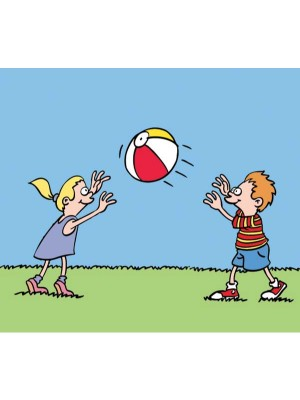
\includegraphics[width=16em,trim=0 0 0 -3]{figures/I21.jpg} & & 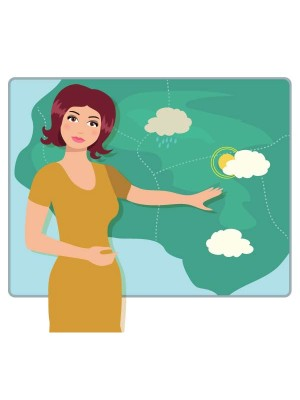
\includegraphics[width=16em,trim=0 0 0 -3]{figures/I22.jpg} \\
\hline
\end{tabular}
\vspace{1em} \\


\begin{tabular}{|c|c|c|}
\hline
23 (Di): What is the doctor doing? && 24 (In): What is the boy doing? \\
\hline

\includegraphics[width=16em,trim=0 0 0 -3]{figures/I23.jpg} & & 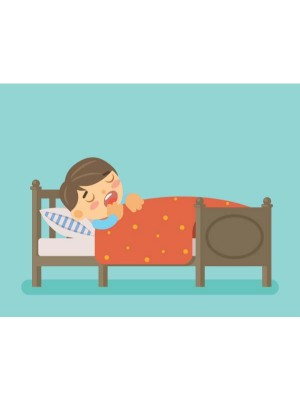
\includegraphics[width=16em,trim=0 0 0 -3]{figures/I24.jpg} \\
\hline
\end{tabular}
\vspace{1em} \\


\clearpage

{\Large \textbf{PDT Items}}

\vspace{2em}

\begin{tabular}{|c|c|c|}
\hline
25 (Tr): What is the dog doing? && 26 (Di): What is the man doing? \\
\hline

\includegraphics[width=16em,trim=0 0 0 -3]{figures/I25.jpg} & & 
\includegraphics[width=16em,trim=0 0 0 -3]{figures/I26.jpg} \\
\hline
\end{tabular}
\vspace{1em} \\


\begin{tabular}{|c|c|c|}
\hline
27 (In): What is the girl doing? && 28 (Di): What is the man doing? \\
\hline

\includegraphics[width=16em,trim=0 0 0 -3]{figures/I27.jpg} & & 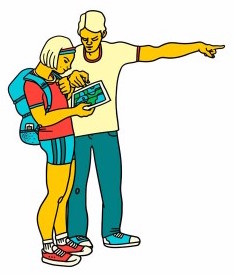
\includegraphics[width=16em,trim=0 0 0 -3]{figures/I28.jpg} \\
\hline
\end{tabular}
\vspace{1em} \\


\clearpage

{\Large \textbf{PDT Items}}

\vspace{2em}

\begin{tabular}{|c|c|c|}
\hline
29 (Tr): What is the woman doing? && 30 (In): What is the woman doing? \\
\hline

\includegraphics[width=16em,trim=0 0 0 -3]{figures/I29.jpg} & & 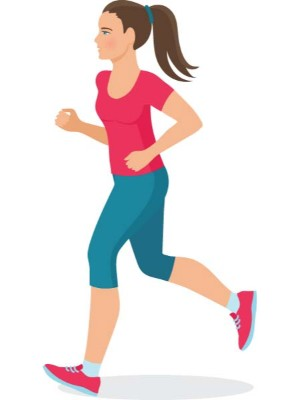
\includegraphics[width=16em,trim=0 0 0 -3]{figures/I30.jpg} \\
\hline
\end{tabular}
\end{center}

\end{document}